Unlike other Machine Learning algorithm applications to systems  and problem, stock trading belongs to a particular branch of algorithm implementation: sequence prediction problems, which tend to prediction of current and next values depends on the history and past records, events do not occur independently. For these situations RNN\footnote{Recurrent Neural Networks, is a class of artificial neural networks where connections between nodes form a directed graph along a temporal sequence\cite{christopher_olah_understanding_2015}}  algorithms are applied to the cryptocurrency candlestick data set\cite{mittal_understanding_2019}.

On the other hand, for the news feed data set it was decided to implement NLP\footnote{Natural Language Processing} algorithms and clustering for unclassified text, since the data set is not labeled. The intention of such classification was to better understand the topics for the news, to isolate, classify them and try to find a pattern to categorize the news. Subsequently a sentiment analysis algorithm can be performed to generate a label that determines whether a specific article is positive or negative, and how meaningful it is for the trading in during the next hours or days. The assumption is that by this results forecasts can be more accurate as they can take articles in real time and merge them with the candlestick data to adapt the training model into a more realistic prediction.

\begin{figure}[H]
   \centering
   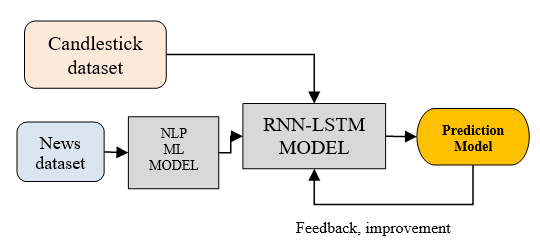
\includegraphics[width=\linewidth]{fig/RNNLSTM.png}
    \caption{ML Training model prototype}
    \label{fig:RNNLSTM}
\end{figure}

\subsection{Cryptocurrency analysis algorithm}

Memory-based networks such as Recurrent Neural Networks (RNN) and Long Short-Term Memory (LSTM) networks allow for predictions to be remembered and forgotten; this can be useful when predicting extreme changes in a short space of time via the remembering of previous examples. Compared to other models, RNN and LSTM are suited towards sequential data such as stock prices, whereas other models must take a non-sequential, sample-independent interpretation of the data, considering only a single input and output sample at a time \cite{chen_lstm-based_2015}

\begin{figure}[H]
   \centering
   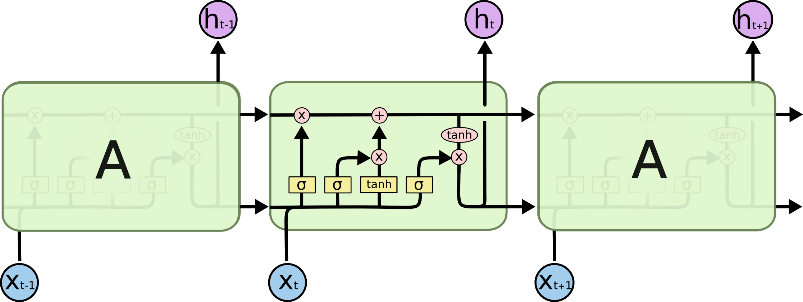
\includegraphics[width=\linewidth]{fig/RNNLSTM2.png}
    \caption{Example of a RNN-LSTM model}
    \label{fig:RNNLSTM2}
\end{figure}

To implement RNN-LSTM approach the python TensorFlow\footnote{TensorFlow is a free and open-source software library for dataflow and differentiable programming across a range of tasks. It is a symbolic math library, and is also used for machine learning applications such as neural networks. Package can be downloaded from \hyperref[https://www.tensorflow.org]{https://www.tensorflow.org}}  deep learning model package was used and adjusted for the best-case scenario in which the loss function and consequent prediction were as accurate as possible without much overfitting. Several examples were observed, the model was retrained for all the cryptocurrency assets using spark functionality with Hadoop ass a file system \cite{yacoub_ahmed_predicting_2019}. 

\subsection{Text and technical sentiment analysis algorithm}

News data set was intended to be classified and processed by using Natural Language processing tools and algorithms to find patterns in the whole dataset. Normal processes for NLP processing require (among others):
\begin{itemize}
    \item String tokenization
    \item Stop words removal
    \item Lexicon normalization
    \item Lemmatization method was applied
    \item Word2Vet approach implemented as well
\end{itemize}

Several NLP and sentiment analysis algorithms were used to classify the model and try obtaining the news topics:

\begin{itemize}
    \item K-Means Clustering
    \item Treating with an unlabeled data set for cryptocurrency news required a machine learning model to try to process and generate corresponding clusters in order to identify the main topics
    \item Sentiment analysis
    \item Common sentiment analysis was performed over the full dataset. This approach aimed to find and tag an approximate positive, neutral or negative sentiment to each document.
    \item Pre-Trained data models
    \item The existence of complex machine learning models based on big scientific documents were used to try to identify and label each article
    \item Text summarization
    \item Extractive summarization approach was performed to try to identify the main topics

\end{itemize}

